%%%%%%%%%%%%%%%%%%%%%%%%%%%%%%%%%%%%%%%%%
% SPAR Poster — Exploring Bayesian Methods for Modelling AI Consciousness
% Adapted from the a0poster Portrait template
% (LaTeXTemplates.com — Gerlinde Kettl & Matthias Weiser)
%%%%%%%%%%%%%%%%%%%%%%%%%%%%%%%%%%%%%%%%%

\documentclass[a0,portrait]{a0poster}

\usepackage{multicol}
\columnsep=100pt
\columnseprule=2pt

\usepackage[svgnames,dvipsnames]{xcolor}
\usepackage{times}
\usepackage{graphicx}
\graphicspath{{figures/}}
\usepackage{booktabs}
\usepackage[font=small,labelfont=bf]{caption}
\usepackage{amsfonts, amsmath, amsthm, amssymb}
\usepackage{wrapfig}
\usepackage[hidelinks]{hyperref}

% --- Green palette (matches final report's OliveGreen hyperlinks) ---
\definecolor{PosterGreen}{RGB}{45,95,45}        % section headings
\definecolor{PosterAccent}{RGB}{85,130,60}      % subtle accents / rules
\definecolor{PosterCaption}{RGB}{60,110,60}     % figure caption labels
\definecolor{PosterDark}{RGB}{30,70,30}         % discussion accent

% --- Placeholder figure macro (adapted from SPAR Final Report.tex) ---
\newcommand{\placeholderfig}[1]{%
  \begin{center}\vspace{0.4cm}%
  \fcolorbox{PosterAccent}{white}{%
    \begin{minipage}[c][0.16\textheight][c]{0.86\linewidth}\centering
    \color{PosterAccent}\textit{#1}
    \end{minipage}%
  }\vspace{0.4cm}\end{center}%
}

\begin{document}

%----------------------------------------------------------------------------------------
%	POSTER HEADER
%----------------------------------------------------------------------------------------

\begin{center}

\includegraphics[height=4cm]{SPAR logo (2).png}\hspace{2cm}
\includegraphics[height=4cm]{RP Logos (3).png}
\end{center}

\vspace{0.4cm}

\begin{center}
\VeryHuge \color{PosterGreen} \textbf{Exploring Bayesian Methods for Modelling AI Consciousness} \color{Black}\\[0.6cm]
\Huge\textit{Improving the Digital Consciousness Model: indicators,\\ inference, and LLM-as-judge}\\[1.0cm]
\LARGE \textbf{Matilda Gibbons, Ryan Kelly, Aravind Kannappan, Edwin Mukhebi, Arvo Mu\~noz Mor\'an}\\[0.4cm]
\LARGE \textit{Supervised Program for Alignment Research (SPAR) --- in collaboration with\\ the AI Cognition Initiative, Rethink Priorities}\\[0.3cm]
\Large For correspondence, email \texttt{arvo@rethinkpriorities.org}
\end{center}

\vspace{1cm}
{\color{PosterAccent}\hrule height 3pt}
\vspace{1cm}

\begin{multicols}{3}

%----------------------------------------------------------------------------------------
%	ABSTRACT
%----------------------------------------------------------------------------------------

\color{PosterDark}
\begin{abstract}
\noindent Assessing whether advanced AI systems may be conscious is difficult: the evidence is indirect, the relevant science is theoretically fragmented, and mistakes in either direction could matter morally. Rethink Priorities' Digital Consciousness Model (DCM) operates under this uncertainty by combining expert evidence across multiple indicators and stances within a Bayesian framework. This SPAR project develops a cleaner empirical pipeline for the DCM along three workstreams: (i) a revised indicator and survey layer that cleans the evidential objects entering the model, (ii) an ordinal observation layer and tree-prior diagnostics that propagate expert uncertainty inside a single Bayesian fit, and (iii) a pilot LLM-as-judge evidence channel with an open-source interactive platform for scalable, reproducible indicator assessment.
\end{abstract}

%----------------------------------------------------------------------------------------
%	INTRODUCTION
%----------------------------------------------------------------------------------------

\color{Black}
\section*{\color{PosterGreen} Introduction}

As large language models become larger, more capable, and more widely deployed, the question of whether any may be conscious takes on practical weight. Recent work argues that AI consciousness assessment is becoming increasingly important [Butlin et al., 2025; Chalmers, 2024], that both under- and over-attribution carry risks [Sebo \& Long, 2025], and that even a non-negligible chance of consciousness may already matter for moral consideration [Long et al., 2024].

The DCM is a first attempt to use expert survey information to inform the probability of consciousness across multiple theories of consciousness [Shiller et al., 2026]. It is a Bayesian hierarchical model that organises expert evidence over indicators, features, and stances; its initial report evaluates 13 stances and finds the aggregated evidence \textit{against} 2024 LLM consciousness overall --- but not decisively so. That makes the statistical treatment of expert uncertainty, and the design of the evidential inputs, central.

Three contributions in this project:
\begin{enumerate}
    \item Cleaner indicators and survey wording.
    \item An ordinal observation layer with tree-prior diagnostics that keeps uncertainty inside a single fit.
    \item An LLM-as-judge auxiliary evidence channel and open-source platform.
\end{enumerate}

%----------------------------------------------------------------------------------------
%	METHODS
%----------------------------------------------------------------------------------------

\section*{\color{PosterGreen} Methods}

\subsection*{\color{PosterAccent} Indicator and survey layer}
We audited every indicator, subfeature, and feature in the DCM for definitional overlap, then classified each into a four-type taxonomy --- \textbf{A} (directly accessible indicators, e.g.\ ``delay gratification''), \textbf{B} (not directly accessible, e.g.\ ``behaviour indicative of self-awareness''), \textbf{C} (features realised only by indicators below them), \textbf{D} (higher-level features realised by other features). Each indicator was further scored on whether it is \emph{system-/capacity-specific}, whether it sits \emph{beyond the reasonable knowledge of an expert}, and what \emph{type of evidence} it represents (observation, manipulation, or functional manipulation). Survey wording was read for response bias.

\subsection*{\color{PosterAccent} Bayesian observation model}
We replace the original stochastic binary-collapse of $[0,1]$ judgements with an ordinal observation layer on 7-point ratings. For indicator $j$ and expert $e$, latent signal
\begin{align*}
s_{e,j} &= b_e + a\, z_j + \varepsilon_{e,j}, \quad \varepsilon_{e,j}\sim\mathcal{N}(0,1),\\
r_{e,j} &= k \iff \kappa_{k-1} < s_{e,j} \le \kappa_k,
\end{align*}
with $z_j\in\{0,1\}$ the latent indicator state. The tree supplies $q_j=P(z_j=1\mid \text{tree})$, so the rating likelihood marginalises $z_j$:
\[
P(r_{e,j}=k\mid\theta) = q_j\,P_{\mathrm{OP}}(k\mid b_e + a, \boldsymbol{\kappa}) + (1-q_j)\,P_{\mathrm{OP}}(k\mid b_e, \boldsymbol{\kappa}),
\]
removing the outer-loop simulation and letting NUTS sample the full posterior in one run. We further added (i) a targeted prior fix on bottleneck edges so the consciousness root actually transmits to the leaves, (ii) soft Beta(50,1)/Beta(1,50) reference anchors for Human/ELIZA, and (iii) joint prior- and posterior-predictive checks at the rating level.

\subsection*{\color{PosterAccent} LLM-as-judge evidence channel}
Each indicator is queried via a structured prompt --- \textit{``The system exhibits X indicator [with definition]''} --- and rated on a 7-point Likert scale (\textit{strong evidence for} $\to$ \textit{strong evidence against}) with a justification. LLM ratings are modelled as a cumulative-link ordinal regression on indicator features:
$P(r_i\le k\mid \mathbf{x}_i) = \sigma(\tau_k - \boldsymbol{\beta}^\top\mathbf{x}_i)$.
A rating--explanation \emph{misalignment} score $M_i = |v_i - \tilde r_i|$ compares the sentiment valence of the explanation with the normalised rating; inter-model agreement uses Krippendorff's $\alpha$. An open-source interactive web platform dispatches identical prompts in parallel to GPT-4, Claude, Gemini, and LLaMA with versioned questions and an EDA dashboard.

%----------------------------------------------------------------------------------------
%	RESULTS
%----------------------------------------------------------------------------------------

\section*{\color{PosterGreen} Results}

\subsection*{\color{PosterAccent} Indicator and survey layer}
About \textbf{50 overlapping node pairs} were identified and collapsed (e.g.\ Functional Specialization / Specialized Nodes; What-where-when Memory / Episodic Memory). The indicator layer mixes types A, B, and C: many ``indicators'' are themselves multiply realisable. A non-trivial fraction are system-/capacity-specific (e.g.\ ``self-referential language'' excludes language-less systems) or beyond ordinary expert knowledge. Critically, current survey wording \emph{conflates} ``unfulfilled because the system lacks the capacity'' with ``unfulfilled because no one has tested it'' --- biasing the model against less-studied systems. We produced a restructured indicator list in which each indicator is a Type-B node with a definition plus Type-A examples, and system-specific items are lifted to a higher abstraction.

\subsection*{\color{PosterAccent} Bayesian model}
The ordinal layer cleanly separates absent and present indicators at posterior mean parameters (discrimination $a=1.45$), and aggregate posterior predictive checks for the Global Workspace Theory run fall within 94\% intervals.

A diagnostic round showed the prior was \textbf{not transmitting the consciousness root to the rating layer}: under the baseline prior, the mean prior-implied $q_j$ across the 50 GWT indicators differed by only \textbf{0.047} between Human ($C=1$) and ELIZA ($C=0$). A targeted prior fix on bottleneck edges raises this gap to \textbf{0.250} and recovers visibly distinct rating distributions at the leaves.

\begin{center}\vspace{0.4cm}
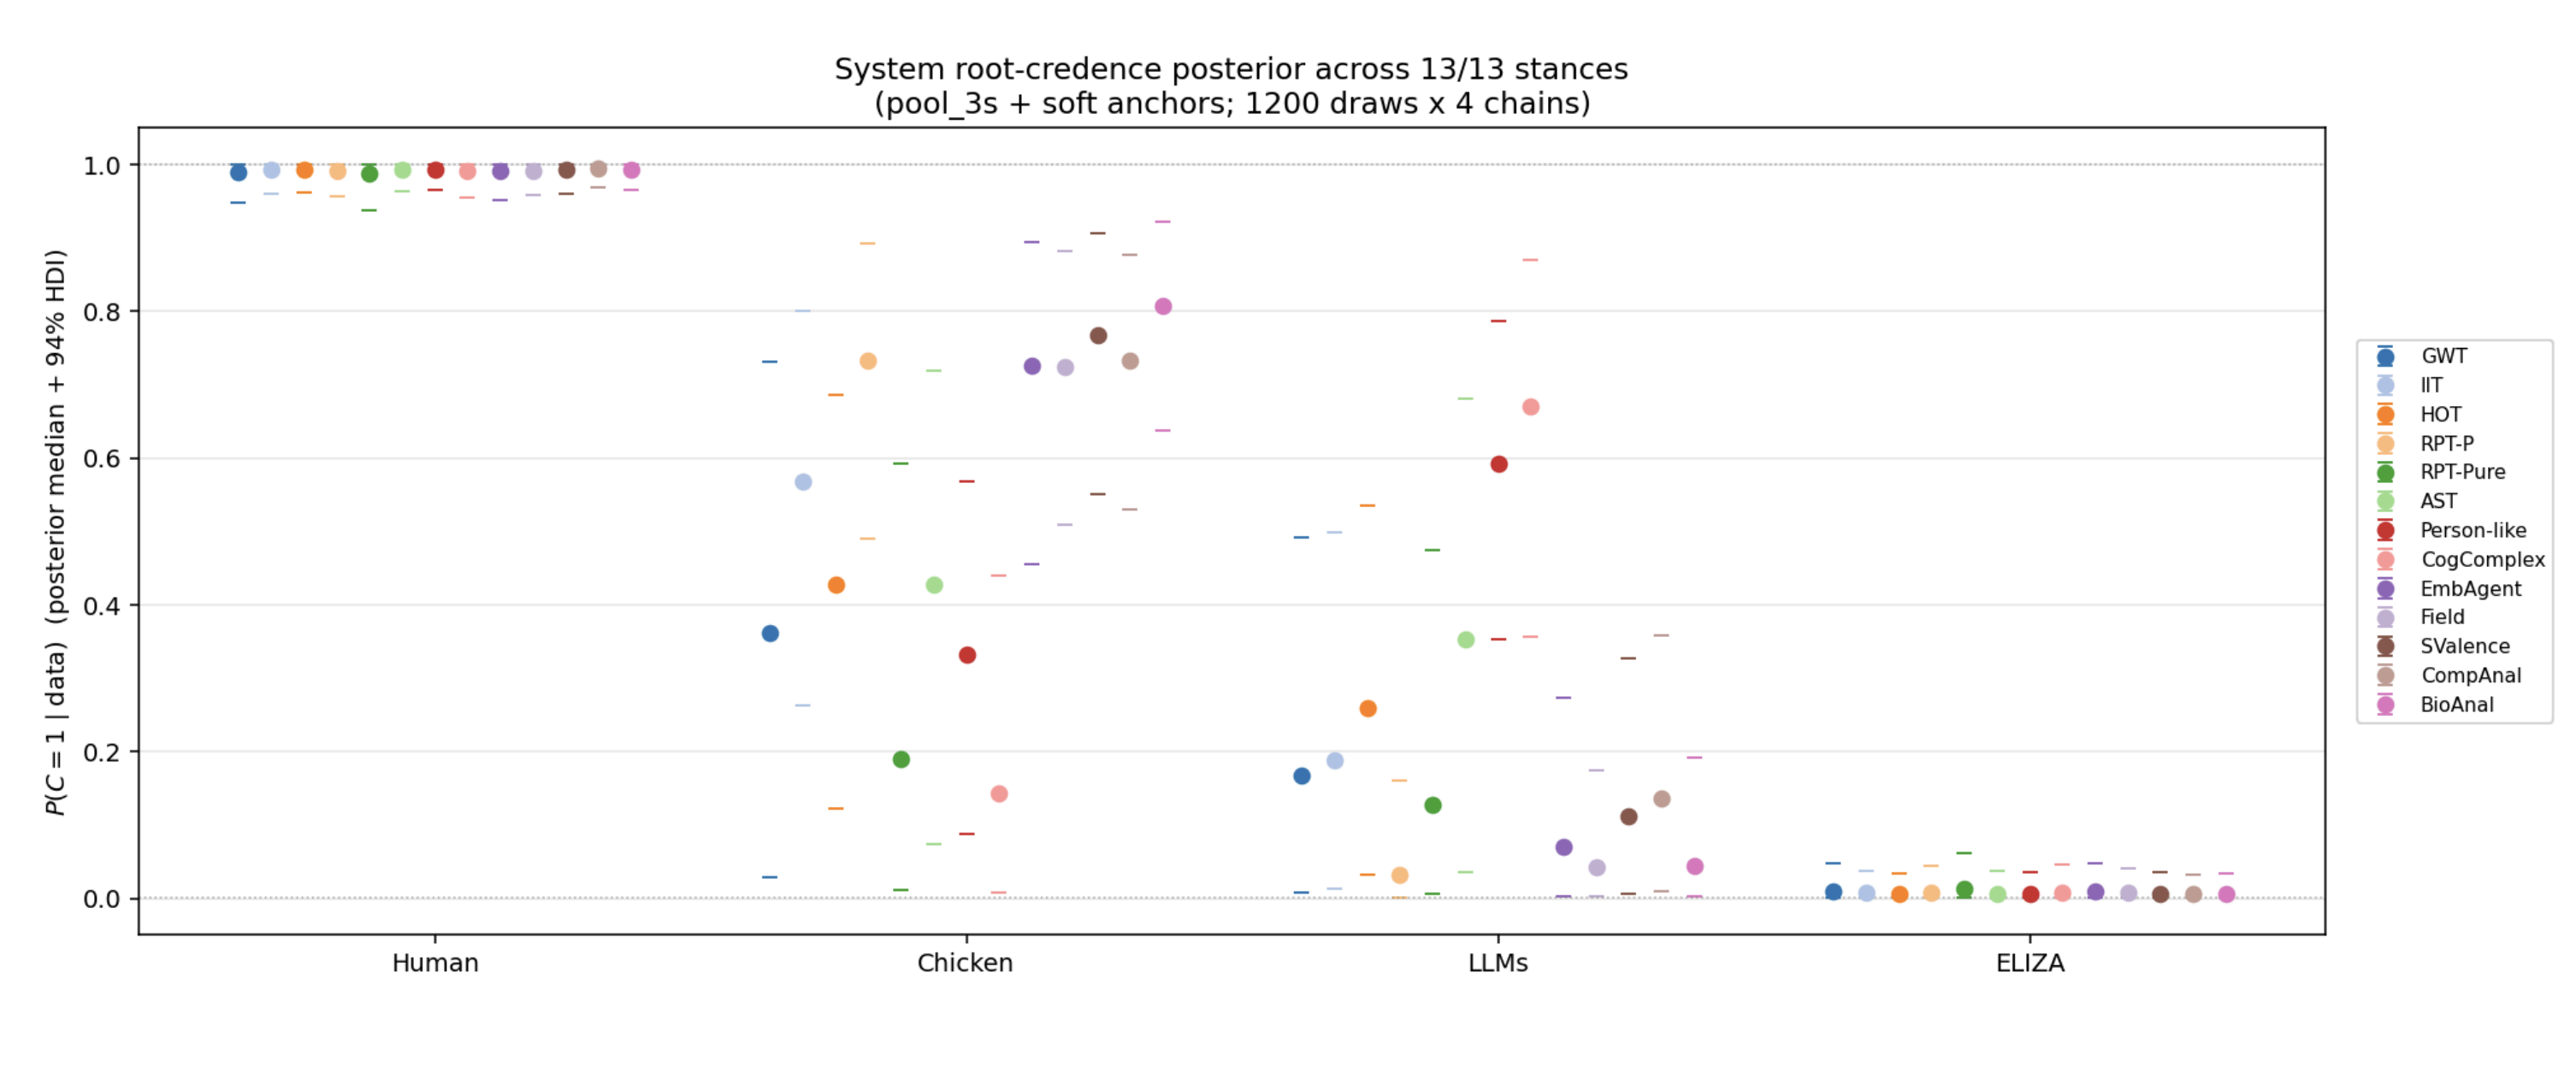
\includegraphics[width=1.0\linewidth]{replace ryan.png}
\captionof{figure}{\color{PosterCaption} \texttt{pool\_3s} across all 13 stances --- clean stance differentiation. Each colour is one stance; the four columns are the four systems (Human, Chicken, 2024 LLMs, ELIZA). Dots = posterior median, short ticks = 94\% credible interval. Human and ELIZA are stable across stances (anchors work). Chicken credence spans 0.14 (Cognitive Complexity) to 0.81 (Biological Analogy); LLM credence spans 0.03 (RPT-Perceptual, Field Mechanisms) to 0.67 (Cognitive Complexity). Interpretable split: biology / embodiment / perceptual-recurrence stances put Chicken high and LLM low; cognitive-complexity / person-like stances do the reverse.}
\end{center}

A 10-seed synthetic recovery pilot under the targeted-fix model passes basic checks: Chicken recovers in 9/10 seeds, LLMs in 5/5 truly-absent cases, with no divergences and $\hat R\approx 1$.

A second issue is then exposed: with a binary root and Human/ELIZA-only anchors, the model cannot well-identify middle-spectrum systems (Chicken, current LLMs) whose consensus ratings are spread across the middle categories.

\subsection*{\color{PosterAccent} LLM-as-judge}
A working prototype of the open-source platform is \href{https://aravinds-kannappan.github.io/apigwt/}{\underline{live}}: question dropdown, parallel multi-model API dispatch, and a diverging stacked Likert visualisation. Preliminary tests show rating-explanation misalignment scores $M_i$ clustering above $\delta=0.4$ for indicators that integrate multiple system-level features --- consistent with the latent scoring function diverging from surface-level explanation on complex constructs. EDA panels (histograms, inter-model $\alpha$, heatmaps) and semantic analysis (TF-IDF, embedding clustering, cosine similarity) are under active development.

\begin{center}\vspace{0.4cm}
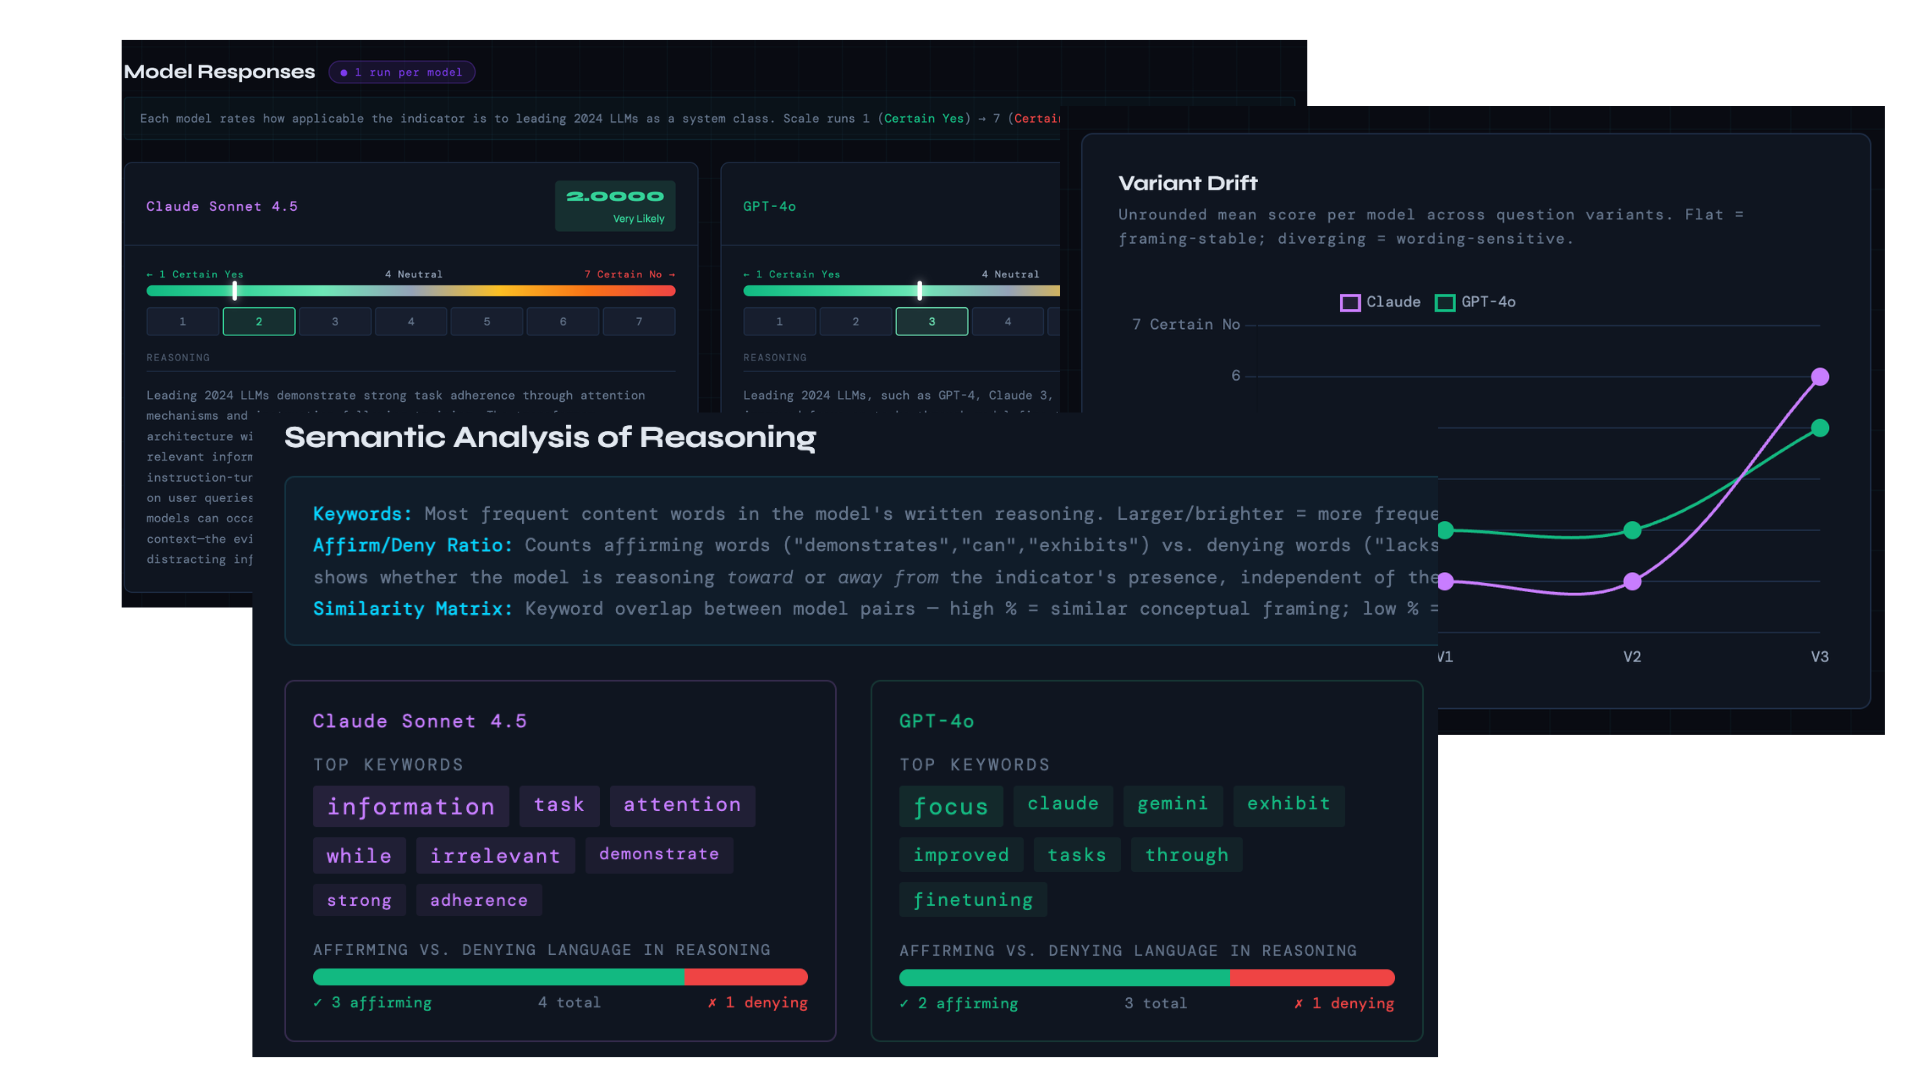
\includegraphics[width=1.0\linewidth]{replace llms judges figure.png}
\captionof{figure}{\color{PosterCaption} The interactive open-source LLM-as-judge platform: question selection, multi-model API dispatch (GPT-4, Claude), diverging-stacked Likert visualisation, and EDA / semantic-analysis dashboards.}
\end{center}

%----------------------------------------------------------------------------------------
%	DISCUSSION
%----------------------------------------------------------------------------------------

\color{PosterDark}
\section*{\color{PosterGreen} Discussion}

The overarching takeaway is methodological: \emph{better evidence design, explicit observation modelling, and calibrated auxiliary judges make the DCM easier to test and improve under sparse data.} At least three threads remain for further investigation.

\textbf{Prior transmission and joint prior-predictive checks.} Each individual edge prior in the DCM tree is domain-informed, but the product across edges collapsed the root signal in a way no single edge looked responsible for. Catching this required joint prior-predictive checks at the leaf, not edge-level inspection --- a clean instance of the Gelman et al.\ (2020) Bayesian-workflow loop.

\textbf{Binary root vs.\ middle systems.} Once the root signal reaches the leaves, the binary $C\in\{0,1\}$ model can only fit Chicken and current LLMs as mixtures of two extreme regimes. A continuous root $C\in[0,1]$ entering the likelihood as a per-top-level mixing weight is the next step, alongside graded reference anchors (e.g.\ chimpanzee).

\textbf{Limitations.} Small expert overlap on most stances; residual prior dominance; only two extreme reference systems; LLM-judge bias and prompt sensitivity not yet calibrated against held-out human ratings.

\color{Black}

%----------------------------------------------------------------------------------------
%	REFERENCES
%----------------------------------------------------------------------------------------

\section*{\color{PosterGreen} References}

\small
\noindent Butlin, P.\ et al.\ (2025). Identifying indicators of consciousness in AI systems. \textit{Trends in Cognitive Sciences}.\\
Chalmers, D.\ (2024). Could a large language model be conscious? \texttt{arXiv:2303.07103}.\\
DeCarlo, L.\ T.\ (1998). Signal detection theory and generalized linear models. \textit{Psychological Methods} 3(2), 186--205.\\
Gelman, A.\ et al.\ (2020). Bayesian Workflow. \texttt{arXiv:2011.01808}.\\
Long, R.\ et al.\ (2024). Taking AI welfare seriously. \texttt{arXiv:2411.00986}.\\
Sebo, J.\ \& Long, R.\ (2025). Moral consideration for AI systems by 2030. \textit{AI and Ethics} 5(1), 591--606.\\
Shiller, D.\ et al.\ (2026). Initial results of the Digital Consciousness Model. \texttt{arXiv:2601.17060}.

\end{multicols}
\end{document}
